\chapter{Model czujnika laserowego}
Istnieje dedykowany obiekt w standardzie SDF dla tego typu czujników.
Również Gazebo wspiera wizualnie symulację poprzez możliwość renderowania zasymulowanych impulsów lasera.
Tak, jak model platformy, ten pakiet otrzymał nazwę kodową \texttt{Monokl}.

\section{Obliczenia symulatora}
	Czujnik laserowy jest bardzo łatwo zasymulować w przestrzeni wirtualnej za pomocą rzutowania półprostych.
	Jest to jedna z podstawowych technik renderowania obrazu.
	Używa się jej także przy obliczaniu symulacji fizycznej i specjalnych wydarzeń związanych, na przykład, z grami komputerowymi.

	Półprosta jest emitowana z jakiegoś punktu w jakimś kierunku w przestrzeni trójwymiarowej.
	Następnie system próbuje znaleźć pierwszy punkt jej kolizji z jakimś symulowanym ciałem fizycznym, posiadającym odpowiedni kolider 
	Ponieważ zasoby komputera zawsze są ograniczone, symulacja półprostej także musi mieć pewien limit. 
	Zwykle jest on jednak na tyle duży, że z punktu widzenia lokalnych wydarzeń, można uznać tą odległość za nieskończoną.

	Algorytm obliczania kolizji z półprostą bazuje na kosztowym porównywaniu pozycji każdego obiektu fizycznego na scenie.
	Istnieją oczywiście sposoby na zmniejszenie ilości obliczeń, na przykład metoda prostopadłościanów zawierających obiekt, ale sposób radzenia sobie z tym nie jest
	częścią tematu pracy,
	Wystarczy wspomnieć, że symulacja dużej ilości laserów jest operacją kosztowną.

\section{Różnice między czujnikiem, a modelem}
	Półprosta emitowana jest z puntu reprezentującego środek czujnika, naturalnie, model upraszcza rzeczywisty czujnik (budowa czujnika laserowego została opisana w sekcji \ref{sec:lidar}).
	Uproszczenie polega na tym, że nie ma w środku żadnego lustra lub obracającej się części. 
	W rzeczywistości w czujniku jest jeden laser, emitujący pulsy w określonych odstępach czasu.
	W modelu można zatem przyjąć osobne półproste dla każdego pulsu lasera.

	Można zauważyć tym samym, że model wydaje się lepszym czujnikiem, niż rzeczywisty LiDAR.
	W danej chwili model emituje promień we wszystkich kierunkach jednocześnie, podczas gdy czujnik jednym pulsem może dokonać tylko jednego pomiaru o danym w tej chwili kącie.
	Jednakże dyskretny sposób symulacji powoduje, że w obu przypadkach dane są podawane w grupach.
	Czujnik jest wstanie wysłać pakiet z danymi ostatniego pomiaru, podczas gdy program modelujący czujnik jest obsługiwany na zasadzie przerwań czasowych 
	po każdej klatce i tylko wtedy może wywołać funkcje zwracające dane zasymulowanych pomiarów.
	To oznacza, że interfejsy do ich obsługi wcale nie różnią się tak bardzo.

	Drugą rzeczą, w której czujnik przoduje, jest nieskończona (z punktu widzenia symulacji) odległość pomiaru.
	Nie tylko jako najdalszy wykryty punkt, ale także i najbliższy. 
	Czujnik nie obcina pomiarów przy określonej odległości, po prostu spada ich jakość, zmniejsza dokładność, zwiększa ilość błędów.
	Symulator ma całkowitą dowolność w ustawianiu progu, dla którego obcina pomiar.

	Podobnie, jak w poprzednim przypadku, symulator zawsze ma taką samą dokładność pomiaru, niezależnie od odległości punktu od czujnika.
	Czujnik zmienia błędność danych w zależności jak daleko od niego jest obiekt.

	W zależności od obciążenia komputera, model czujnika jest podatny na opóźnienia w odczytywaniu stanu.
	Czujnik zawsze działa z tą samą częstotliwością, a jego program sterujący jest wbudowany w mikrokontroler i spełnia sztywne ramy czasowe.

\section{Komunikacja}
	Jednakże, bazując na architekturze opisanej wcześniej na rysunku \ref{fig:agent}, należy tak zbudować system, aby program komunikował się w identyczny sposób z 
	modelem czujnika, jak i samym czujnikiem.
	Służą do tego specjalne pakiety ROSa, zawierające czas pomiaru, typ i dane.
	Program obsługujący model czujnika generuje i wysyła pakiety typu \texttt{sensor\_msgs/LaserScan}.

	Identycznie, inny program, podłączony do czujnika za pomocą jednego z interfejsów, także powinien generować takie same pakiety.

\section{Model w Gazebo}
	Tak, jak w modelu platformy, należy stworzyć odpowiedni dokument SDF. 
	Aby umożliwić przenoszenie modelu czujnika na modele innych platform, powinien on być niezależny od implementacji platformy do której będzie przytwierdzony.
	Dodatkowo, w końcowym modelu istnieć będą dwa takie czujniki.

	Model składa się z dwóch elementów: korpusu i samego ,,mechanizmu'' urządzenia.
	Mechanizm przytwierdzony jest w odpowiednim miejscu korpusu za pomocą stałego połączenia (elementu \texttt{joint}).

	Korpus posiada siatkę, reprezentującą uproszczony wygląd urządzenia, a także dwa elementy w kształcie walców, odpowiedzialne za kolizję.
	Odpowiada za przesunięcie samego lasera względem podstawy na której całe urządzenie jest montowane i pozwala na wygodną referencję z innego modelu w celu utworzenia połączenia.

	Główna część czujnika posiada ozdobną siatkę udającą czarną szybkę LiDARa, oraz element SDF \texttt{sensor}, odpowiedzialny za sam czujnik.
	W kolejnych podelementach zawierają się parametry urządzenia, takie jak ilość symulowanych laserów, ich zasięg, kąt pierwszego i ostatniego lasera, oraz współczynnik błędu pomiarowego.
	
	Teoretycznie, lepiej aby model posiadał jeden element odpowiedzialny za kolizje, gdyż to byłoby szybsze do symulacji. 
	Jednakże, półproste emitowane ze środka również się by z nim zderzały, a co za tym idzie, nie opuszczałyby modelu czujnika.
	Dlatego potrzeba jest, aby w miejscu ich wychodzenia (czarna szybka) nie było żadnego koldera.

	\subsection{Połączenie modeli}
		Jak wcześniej wspomniano,
		%TODO gdzie?
		model SDF ma strukturę gwiaździstą. 
		Zagnieżdżenie modeli spowodowałoby, że powstaje inna struktura, drzewiasta.
		Dlatego też, element \texttt{import} nie umieszcza w swoim miejscu całego modelu z innego pliku, a raczej importuje jego składowe i umieszcza równolegle do istniejących.
		To oznacza, że zadbać trzeba także o elementy \texttt{joint}, łączące element podstawy platformy z podstawą czujnika, inaczej symulacja widziałaby dwa osobne modele.
		Więc potrzebna jest także znajomość nazw elementów składowych importowanego modelu.

		Taka mechanika działania wydaje się mało zrozumiała i nieintuicyjna, jednak doskonale dba o zachowanie spójności modelu.
		Wszystko nadal pozostaje gwiazdą i każdy element musi być odpowiednio połączony z pozostałymi, aby dokładnie określić fizykę interakcji.
		Nie powstają sytuacje w których zachowanie jakichś elementów będzie niezrozumiałe.

		Ma to także swoją wadę. Importując dwa, identyczne modele, ich składowe tracą informację o swoich wspólnych rodzicach.
		Program sterujący czujnikiem nie ma sposoby sprawdzić, którym czujnikiem steruje, a co za tym idzie, jaką nazwę interfejsu wystawić do nadawania wiadomości.
		Jedynym sposobem na rozwiązanie tego problemu jest nadanie importowanym elementom różnych przedrostków do nazw.
		I także sterownik musi tylko na tej podstawie określić czujnik, w którym jest.

		Alternatywnie, zawsze można stworzyć dwa, osobne modele czujników, albo wszystko umieścić od razu w jednym pliku.
		Jednak takie rozwiązanie niszczy komponentową budowę środowiska i nie pozwala na użycie składowych w innych modelach.
		
		\begin{figure}[h]
		\centering
		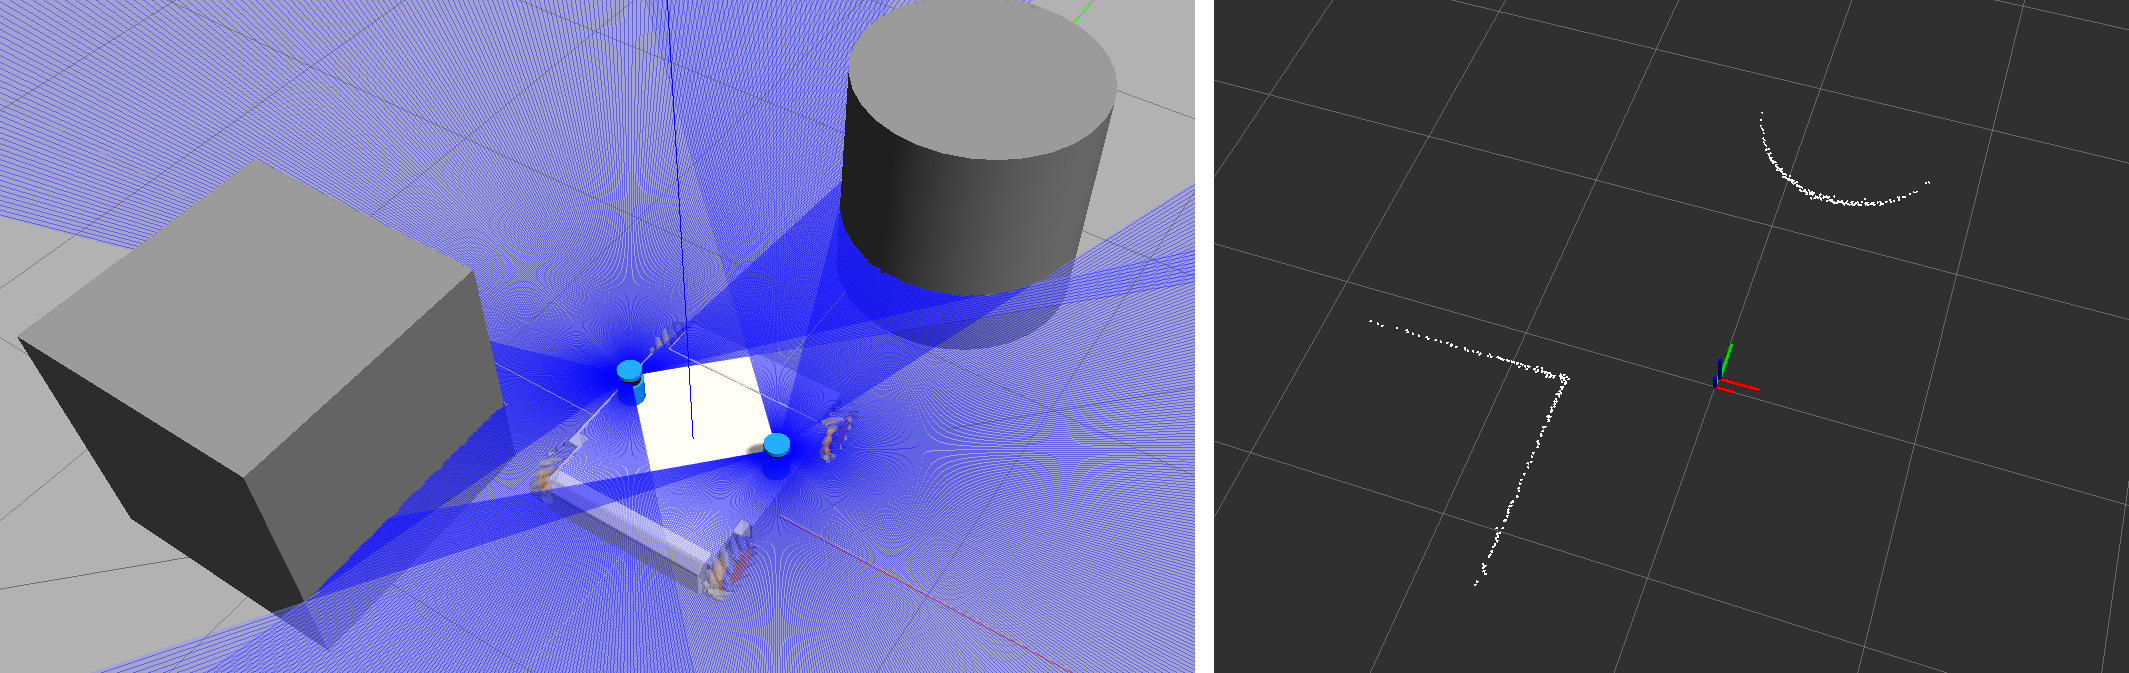
\includegraphics[width=\textwidth]{graphics/scan.png}
		\caption{Zrzut ekranu platformy z Gazebo i wygenerowane dane, obserwowane w Rviz.}
		\label{fig:scan}
		\end{figure}
		
	\subsection{Mechanika ramek}
		\label{sec:frames}
		Komunikacja poprzez pakiety wiadomości nie jest jedynym sposobem na przekazywanie informacji w środowisku ROS.
		%TODO wspomnieć o tym wcześniej
		Istnieje także mechanika ramek transformacji \texttt{TF2}.
		Jest to podobna rzecz do niezaimplementowanej funkcjonalności Gazebo, ale nie jest automatyczna i nie ogranicza się tylko do jednego programu.
		
		Ramka transformacji jest informacją o aktualnej pozycji i rotacji jakiegoś obiektu względem innego.
		Polega na wysłaniu pakietu typu \texttt{geometry\_msgs/TransformStamped} prosto do demona ROS.
		Pakiet zawiera w sobie nagłówek, informujący o czasie i identyfikatorze nadania ramki, i względem jakiego obiektu podawana jest pozycja i rotacja.
		Następna jest nazwa nowej ramki, jej pozycja i rotacja względem nazwy obiektu podanego w nagłówku.
		Dowolny program może nadać dowolny pakiet transformacji.
		Demon ROSa następnie zbiera wszystkie pozycje i oblicza transformacje dla programów, które pytają się o względne pozycje elementów.
		
		Przykładowo, gdyby symulacja robota nie odbywałaby się w przestrzeni wirtualnej, w maszynie symulacyjnej fizyki, 
		informacja o dokładnym położeniu obiektu składowego w przestrzeni wcale nie musiałaby być tak łatwo dostępna.
		To ma szczególne znaczenie dla skomplikowanych mechanizmów typu wielosegmentowe ramię manipulacyjne.
		Obliczenie pozycji i rotacji końcówki ramienia wymagałoby informacji o aktualnych pozycjach i rotacjach wszystkich innych segmentów.
		Która strona miałaby zajmować się obliczeniami i kto powinien posiadać i komu przekazywać te informacje?
		
		Demon ROSa działa tutaj jak trzecia strona, zbierająca dane od przegubów i obliczająca pozycje i rotacje wszystkich punktów.
		W takim przypadku, każdy segment symulacji mógłby przekazywać swój identyfikator, identyfikator obiektu którym steruje, jego pozycję i rotację.
		Inne programy, na przykład do wizualizacji, mogłyby wtedy zapytać się demona ROSa o dokładne pozycje przegubów w przestrzeni kartezjańskiej, a on obliczyłby je i zwrócił.
		
		W symulacji platformy wielokierunkowej mechanika ramek jest potrzebna, gdyż pakiet zwierający pomiary z czujnika laserowego nie posiada informacji o aktualnej
		pozycji samego czujnika, a jedynie identyfikator swojej ramki. Te informacje potrzebne są programowi obliczającemu pozycję z czujników i ewentualnemu wizualizatorowi samych
		czujników laserowych.
		
		Symulator platformy zawiera drugi program, który w każdym cyklu symulacji nadaje demonowi ROSa pozycje i rotacje środków czujników laserowych, dla uproszczenia
		względem początku układu współrzędnych, punktu (0,0,0). 
		Program sterujący modelem samej platformy także nadaje ramkę z pozycją i rotacją platformy względem środka układu.
		Dokładnie taki sam efekt byłby, gdyby nadawać stałą pozycję i rotację czujników laserowych, ale względem ramki platformy (nadawanej przez inny sterownik).
		Stałą, ponieważ czujniki nie zmieniają swojej pozycji na platformie, są przytwierdzone na stałe.
		
		\begin{table}
			\centering
			\begin{tabular}{l r}
				Punkt ramki & Nazwa punktu \\
				\hline
				Stały środek mapy & \texttt{map} \\
				Środek platformy & \texttt{omnivelma} \\
				Środek platformy kinematycznej & \texttt{pseudovelma} \\
				Emiter prawego lasera & \texttt{monokl\_r\_heart} \\
				Emiter lewego lasera & \texttt{monokl\_l\_heart} \\
			\end{tabular}
			\caption{Nazwy identyfikatorów ramek, używanych w symulatorze.}
			\label{tab:frames}
		\end{table}
			
		\begin{table}
			\centering
			\begin{tabular}{l c r}
				Nazwa & Punkt względny & Punkt danych \\
				\hline
				Pozycja i rotacja platformy & \texttt{map} & \texttt{omnivelma} \\
				Pozycja i rotacja platformy kinematycznej & \texttt{map} & \texttt{pseudovelma} \\
				Pozycja i rotacja prawego czujnika & \texttt{map} & \texttt{monokl\_r\_heart} \\
				Pozycja i rotacja lewego czujnika & \texttt{map} & \texttt{monokl\_l\_heart} \\
			\end{tabular}
			\caption{Ramki wysyłane do demona ROS.}
			\label{tab:frame_send}
		\end{table}

\section{Błędy}
	Jak podano wcześniej w tabelce \ref{tab:lidar}, wyróżnione są dwa typy błędów pomiaru, systematyczny i pomiarowy.
	Dodatkowo istnieje także błąd gruby.
	Model czujnika powinien uwzględniać te błędy, aby zwracać dane jak najbardziej zbliżone do LiDARa.

	\subsection{Błąd gruby}
		Najprostszy typ błędu polega na dużych odchyłach niektórych pomiarów od pozostałych wartości.
		W trakcie przetwarzania odczytu, te punkty powinno się odrzucić.
		Nie mniej jednak, to zadanie należy do programu sterującego, więc należy umożliwić mu testowanie tej funkcjonalności poprzez wprowadzenie takich błędów do zasymulowanych odczytów.

		Najczęstszym przypadkiem błędu grubego jest brak odbioru wysłanego impulsu. 
		To skutkuje nadaniem aktualnemu pomiarowi wartości maksymalnej, co jest bardzo łatwo wykryć i usunąć.

		Innym problemem może być odebranie światła niepochodzącego od emitera urządzenia, a jakiegoś zewnętrznego źródła.

		Ponieważ rozkład i częstotliwość tych błędów zależy od środowiska w jakim działa czujnik, bardzo ciężko jest dobrać odpowiedni algorytm ich generacji.
		%TODO dopisać po implementacji

	\subsection{Błąd systematyczny}
		Ten błąd jest stałą wartością, dodaną do każdego pomiaru.
		Spowodowany jest niedoskonałością budowy elementów pomiarowych, niewłaściwą kalibracją, zużyciem, lub otoczeniem w jakim pracuje czujnik.

		Rzeczywisty czujnik powinien być skalibrowany przed użyciem właśnie po to, aby wewnętrzny program sterujący mógł obliczyć aktualne zboczenia 
		i skorygować pomiary przed wysłaniem ich dalej. Kalibracja może być nadana na samym urządzeniu, poprzez zmianę jego parametrów działania,
		inaczej, zmianę współczynników przy korygowaniu pomiarów, przez system wbudowany, przed wysłaniem.
		Czujnik może także wysyłać czyste i obarczone błędami dane do programu sterującego, który samodzielnie je skoryguje.
		Pozwoli to na zastosowanie dowolnych algorytmów oczyszczania danych, kosztem większego obciążenia programu sterującego.

		Symulator czujnika powinien mieć interfejs do ustawienia tej wartości, aby mógł być ,,skalibrowany'' w taki sam sposób, jak faktyczne urządzenie.
		%TODO dopisać po implementacji

	\subsection{Błąd pomiarowy}
		Jest to mała, losowa wartość, dodana do każdego pomiaru.
		Wynika ona z niedoskonałości samego czujnika, nieznanych zakłóceń i niezbadanych efektów kwantowych.
		Nie da się w żaden sposób usunąć, zmniejszyć, lub przewidzieć tego typu błędów.
		Jedynym sposobem jest obliczenie średniej błędu na podstawie dużej ilości pomiarów.

		Błąd pomiarowy ma zwykle rozkład normalny o określonym odchyleniu standardowym.
		Standard SDF przewiduje element określający tę liczbę, a Gazebo może wewnętrznie obliczyć i dodać do wyników odpowiednią wartość.
		Również producent podał w tabeli danych urządzenia obliczony rozkład standardowy.

		W związku z tym, wartość podana przez producenta, podana w tabelce \ref{tab:lidar}, może być bezpośrednio zapisana do 
		elementu odchylenia standardowego, w pliku SDF opisującym czujnik.
		Wadą takiego rozwiązania jest niemożność modyfikacji tego parametru w trakcie wykonywania programu, gdyż Gazebo nie wystawia API do modyfikacji tej wartości.
		Aby temu zaradzić, wystarczy obliczać błąd standardowy w programie sterującym i manualnie dodawać go do zwróconej przez symulator tablicy.
		Funkcje do obliczania błędu standardowego zostały wprowadzone do standardu języka C++ w 2011 roku.



